\documentclass[12pt,titlepage]{article}
\usepackage[margin=1.25in]{geometry}
\usepackage{graphicx,amsmath,blindtext,minted}

%% Variables definition
\newcommand{\vSubject}{Advance Data Base}
\newcommand{\vSubtitle}{Midterm}
\newcommand{\vName}{Muhammad Baihaqi Aulia Asy'ari}
\newcommand{\vNIM}{2241720145}
\newcommand{\vClass}{2I}
\newcommand{\vDepartment}{Information Technology}
\newcommand{\vStudyProgram}{D4 Informatics Engineering}

%% [START] Tikz related stuff
\usepackage{tikz}
\usetikzlibrary{svg.path,calc,shapes.geometric,shapes.misc}
\tikzstyle{terminator} = [rectangle, draw, text centered, rounded corners = 1em, minimum height=2em]
\tikzstyle{preparation} = [chamfered rectangle, chamfered rectangle sep=0.75em, draw, text centered, minimum height = 2em]
\tikzstyle{process} = [rectangle, draw, text centered, minimum height=2em]
\tikzstyle{decision} = [diamond, aspect=2, draw, text centered, minimum height=2em]
\tikzstyle{data}=[trapezium, draw, text centered, trapezium left angle=60, trapezium right angle=120, minimum height=2em]
\tikzstyle{connector} = [line width=0.25mm,->]
%% [END] Tikz related stuff

%% [START] Fancy header related stuff
\usepackage{fancyhdr}
\pagestyle{fancy}
\setlength{\headheight}{15pt} % compensate fancyhdr style
\fancyhead{}
\fancyfoot{}
\fancyfoot[L]{\thepage}
\fancyfoot[R]{\textit{\vSubject - \vSubtitle}}
\renewcommand{\footrulewidth}{0.4pt}% default is 0pt, overline for footer
%% [END] Fancy header related stuff

%% [START] Custom tabular command related stuff
\usepackage{tabularx}
\newcommand{\details}[2]{
    #1 & #2  \\
}
%% [END] Custom tabular command related stuff

%% [START] Figure related stuff
\newcommand{\image}[3][1]{
    \begin{figure}[h]
        \centering
        \includegraphics[#1]{#2}
        \caption{#3}
        \label{#3}
    \end{figure}
}
%% [END] Figure related stuff

%%
\usepackage{pgf-umlcd}

\renewcommand{\umldrawcolor}{black}
\renewcommand{\umlfillcolor}{white}
%%

%% [BEGIN] Custom enumerator
\usepackage{enumitem}
%% [END] Custom enumerator

%% [BEGIN] Paragraph indent
\usepackage{indentfirst}
%% [END] Paragraph indent

\begin{document}
\begin{titlepage}
    \centering
    \vfill
    {\bfseries\LARGE
        \vSubject\\
        \vskip0.25cm
        \vSubtitle
    }
    \vfill
    
\includegraphics[width=6cm]{images/polinema-logo.png}
    \vfill
    {
        \textbf{Name}\\
        \vName\\
        \vskip0.5cm
        \textbf{NIM}\\
        \vNIM\\
        \vskip0.5cm
        \textbf{Class}\\
        \vClass\\
        \vskip0.5cm
        \textbf{Department}\\
        \vDepartment\\
        \vskip0.5cm
        \textbf{Study Program}\\
        \vStudyProgram
    }
\end{titlepage}

\newpage

\section{Case Study Setup}

\subsection{Create Tables}
\begin{center}
    \includegraphics[width=.85\textwidth]{images/figures/fig1.png}
\end{center}

\subsection{Insert Data}
\begin{center}
    \includegraphics[width=.85\textwidth]{images/figures/fig2.png}
    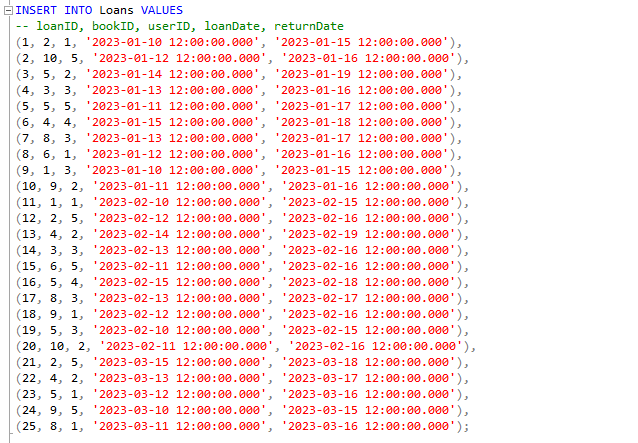
\includegraphics[width=.85\textwidth]{images/figures/fig3.png}
\end{center}

\section{Assignment}

\begin{enumerate}
    \item - \\ \includegraphics[width=.9\textwidth]{images/figures/fig4_a.png} \\ \includegraphics[width=.9\textwidth]{images/figures/fig4_b.png}
    
    \newpage

    \item \texttt{Query} \\ \includegraphics[width=.9\textwidth]{images/figures/fig5_a.png} \\ Result \\ 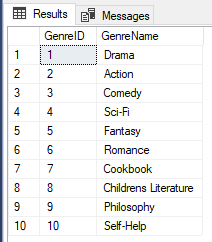
\includegraphics[width=.9\textwidth]{images/figures/fig5_b.png} \\ \includegraphics[width=.9\textwidth]{images/figures/fig5_c.png} \\ 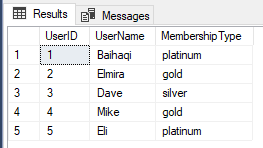
\includegraphics[width=.9\textwidth]{images/figures/fig5_d.png} \\ \includegraphics[width=.9\textwidth]{images/figures/fig5_e.png}
    \item \texttt{Query} \\ \includegraphics[width=.9\textwidth]{images/figures/fig6_a.png} \\ Result \\ \includegraphics[width=.9\textwidth]{images/figures/fig6_b.png}
    \item \texttt{Query} \\ \includegraphics[width=.9\textwidth]{images/figures/fig7_a.png} \\ Result \\ \includegraphics[width=.9\textwidth]{images/figures/fig7_b.png}
    \item \texttt{Query} \\ \includegraphics[width=.9\textwidth]{images/figures/fig8_a.png} \\ Result \\ \includegraphics[width=.9\textwidth]{images/figures/fig8_b.png}
    \item \texttt{Query} \\ \includegraphics[width=.9\textwidth]{images/figures/fig9_a.png} \\ Result \\ \includegraphics[width=.9\textwidth]{images/figures/fig9_b.png}
    \item \texttt{Query} \\ \includegraphics[width=.9\textwidth]{images/figures/fig10_a.png} \\ Result \\ 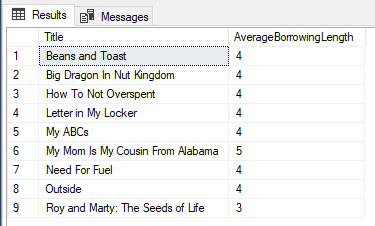
\includegraphics[width=.9\textwidth]{images/figures/fig10_b.png}
    \item \texttt{Query} \\ 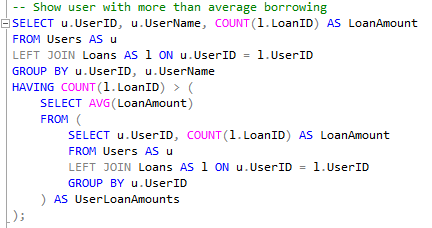
\includegraphics[width=.9\textwidth]{images/figures/fig11_a.png} \\ Result \\ 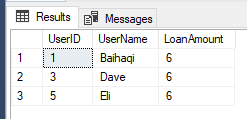
\includegraphics[width=.9\textwidth]{images/figures/fig11_b.png}
    \item \texttt{Query} \\ 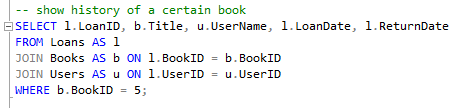
\includegraphics[width=.9\textwidth]{images/figures/fig12_a.png} \\ Result \\ \includegraphics[width=.9\textwidth]{images/figures/fig12_b.png}
    \item \texttt{Query} \\ 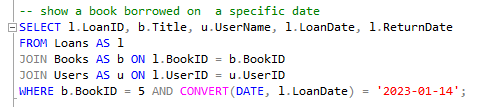
\includegraphics[width=.9\textwidth]{images/figures/fig13_a.png} \\ Result \\ \includegraphics[width=.9\textwidth]{images/figures/fig13_b.png}
    \item \texttt{Query} \\ \includegraphics[width=.9\textwidth]{images/figures/fig14_a.png} \\ Result \\ 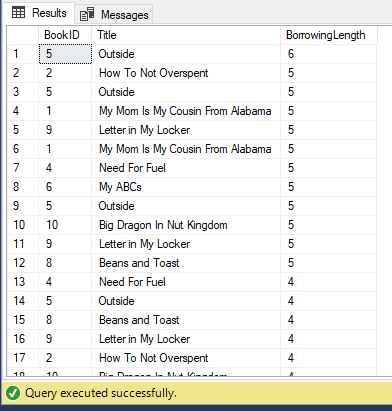
\includegraphics[width=.9\textwidth]{images/figures/fig14_b.png}
    \item \texttt{Query} \\ 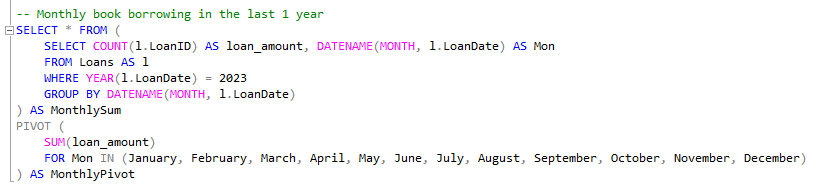
\includegraphics[width=.9\textwidth]{images/figures/fig15_a.png} \\ Result \\ \includegraphics[width=.9\textwidth]{images/figures/fig15_b.png}
\end{enumerate}

\end{document}